\documentclass[english]{kththesis}

\usepackage[style=numeric,sorting=none,backend=biber]{biblatex}
\usepackage[acronym, section=section, nonumberlist, nomain, nopostdot]{glossaries}
\usepackage[perpage,symbol]{footmisc}
\usepackage[parfill]{parskip} % Linebreak paragraphs instead of indent

\usepackage{longtable}
\usepackage{booktabs}
\usepackage{enumitem}

\usepackage{xcolor}     % Remove after \todo has been removed
\usepackage{tabularx}   % For additional table formatting
\usepackage{subcaption} % For subfigure support
\usepackage{pgfmath}    % --math engine
\usepackage{array}      % For table wrapping
\usepackage{graphicx}   % Support for images
\usepackage{float}      % Support for more flexible floating box positioning
\usepackage{setspace}   % For fine-grained control over line spacing
\usepackage{listings}   % For source code listing
\usepackage{tabularx}   % For simple table stretching
\usepackage{multirow}   % Support for multirow colums in tables
\usepackage{url}        % Support for breaking URLs
\usepackage{hyperref}
\usepackage[all]{hypcap}  % prevents an issue related to hyperref and caption linking
%% setup hyperref to use the darkblue color on links
\hypersetup{colorlinks,breaklinks,
            linkcolor=darkblue,urlcolor=darkblue,
            anchorcolor=darkblue,citecolor=darkblue}

%% Some definitions of used colors
\hyphenpenalty=15000\tolerance=1000 % to reduce hyphenation
\definecolor{darkblue}{rgb}{0.0,0.0,0.3} %% define a color called darkblue
\definecolor{darkred}{rgb}{0.4,0.0,0.0}
\definecolor{red}{rgb}{0.7,0.0,0.0}
\definecolor{lightgrey}{rgb}{0.8,0.8,0.8} 
\definecolor{grey}{rgb}{0.6,0.6,0.6}
\definecolor{darkgrey}{rgb}{0.4,0.4,0.4}
\definecolor{aqua}{rgb}{0.0, 1.0, 1.0}

\usepackage[cache=false]{minted} %% For source code highlighting
\usemintedstyle{borland}

\usepackage{csquotes} % Recommended by biblatex

% set the chapter header
\renewcommand{\chaptermark}[1]{\markboth{#1}{}}

% to get rolling footnote numbers
\counterwithout{footnote}{chapter}

\newcolumntype{P}[1]{>{\endgraf\vspace*{-\baselineskip}}p{#1}}

% custom macros
\newcommand{\footnotelink}[2]{\footnote{\url{#1} | Accessed #2}}
\newcommand{\todo}[0]{\colorbox{orange}{TODO}}

% The list of acronyms and abbreviations should be in alphabetical order based on the spelling of the acronym or abbreviation.
\makeglossaries

\newacronym{IOT}{IoT}{Internet of Things}
  
\begin{document}

\date{\today}
\title{A security analysis of SecuritasHome Home Alarm System}
\subtitle{[Todo subtitle]}
\alttitle{En säkerhetsanalys av SecuritasHome hemlarmsystem}
\altsubtitle{[Todo subtitle]}

\authorsLastname{Lindeberg}
\authorsFirstname{Axel}
\email{alindeb@kth.se}
\kthid{alindeb}
\authorsSchool{\schoolAcronym{EECS}}
\programcode{CDATE}

% KTH Supervisor
\supervisorAsLastname{Johnson}
\supervisorAsFirstname{Pontus}
\supervisorAsEmail{pontusj@kth.se}
\supervisorAsKTHID{pontusj}
\supervisorAsSchool{\schoolAcronym{EECS}}
\supervisorAsDepartment{Division of Network and Systems Engineering}

% External Supervisor
%\supervisorBsLastname{[EFTERNAMN]}
%\supervisorBsFirstname{[NAMN]}
%\supervisorBsEmail{temp@fm.se}
%\supervisorBsOrganization{Försvarsmakten}
\hostcompany{Swedish Armed Forces (Försvarsmakten)}

% KTH Examiner
\examinersLastname{Lagerström}
\examinersFirstname{Robert}
\examinersEmail{robertl@kth.se}
\examinersKTHID{robertl}
\examinersSchool{\schoolAcronym{EECS}}
\supervisorAsDepartment{Division of Network and Systems Engineering}

\titlepage
\bookinfopage

\frontmatter
\setcounter{page}{1}

% ---- English Abstract ----
\begin{abstract}
\markboth{\abstractname}{}
% Keep in mind that most of your potential readers are only going to read your title and abstract. This is why it is important that the abstract give them enough information that they can decide is this document relevant to them or not. Otherwise the likely default choice is to ignore the rest of your document.
% A abstract should stand on its own, i.e., no citations, cross references to the body of the document, acronyms must be spelled out, …
% Write this early and revise as necessary. This will help keep you focused on what you are trying to do.

% Write an abstract (250 and 350 words) with the following components:
%  - What is the topic area? (optional) Introduces the subject area for the project.
%  - Short problem statement
%  - Why was this problem worth a Master’s thesis project? (i.e., why is the problem both significant and of a suitable degree of difficulty for a Master’s thesis project? Why has no one else solved it yet?)
%  - How did you solve the problem? What was your method/insight?
%  - Results/Conclusions/Consequences/Impact: What are your key results/conclusions? What will others do based upon your results? What can be done now that you have finished - that could not be done before your thesis project was completed? The presentation of the results should be the main part of the abstract.
\todo

\subsection*{Keywords}
% Choosing good keywords can help others to locate your paper, thesis, dissertation, … and related work.}
% Choose the most specific keyword from those used in your domain, see for example:
% ACM's Computing Classification System (2012) or
% (2014) IEEE Taxonomy. 
% Mechanics:
% - The first letter of a keyword should be set with a capital letter and proper names should be capitalized as usual.
% - Spell out acronyms and abbreviations.
% - Avoid "stop words" - as they generally carry little or no information.
% - List your keywords separated by commas (",").
% Since you should have both English and Swedish keywords - you might think of ordering them in corresponding order (i.e., so that the nth word in each list correspond) - thus it would be easier to mechanically find matching keywords.
\todo

\end{abstract}

% ---- Swedish Abstract ----
\selectlanguage{swedish}
\begin{abstract}
% All theses at KTH are required to have an abstract in both English and Swedish.
% If you are writing your thesis in English, you can leave this until the final version. If you are writing your thesis in Swedish then this should be done first – and you should revise as necessary along the way.
% If you are writing your thesis in English, then this section can be a summary targeted at a more general reader. However, if you are writing your thesis in Swedish, then the reverse is true – your abstract should be for your target audience, while an English summary can be written targeted at a more general audience.
% The Swedish sammanfattning need not be a literal translation of the english abstract.
\todo

\subsection*{Nyckelord}
\todo

\end{abstract}

\clearpage

\selectlanguage{english}
\section*{Acknowledgments}
\markboth{Acknowledgments}{}
I would like to thank Fredrik Heiding, PhD student within cybersecurity at KTH, for helping me procure the alarm system investigated in this thesis, as well as the HackRF SDR, and navigating the KTH bureaucracy surrounding that process.

I would also like to acknowledge Professor Andreas Noack from the University of Applied Sciences Stralsund in Germany. Not only did he co-create the excellent tool \textit{Universal Radio Hacker} which was used extensively in this thesis. He also offered up a lot of his time in personally helping me when I initially felt way out of my depth with RF hacking by answering questions about the URH tool, RF communication in general, and figuring out how to capture good signals for this system.

Next, I would like to thank my girlfriend, Caroline, who had to hear me go on and on about radio waves and RF hacking for months, handle the stressful periods, for continuously proofreading the thesis, and for putting up with this whole situation during a pandemic. The same goes for the rest of my family.

I would, of course, like to thank my supervisor at Försvarsmakten. They gave me invaluable insights and expertise during this entire project. All the way from selecting what type of system to explore, to sharing their knowledge during the pentesting phase, to proofreading the final version. They also lent me more than enough of their time, meeting with me every week to discuss the thesis which I really appreciated.

Above all, I would like to thank my KTH supervisor Pontus Johnson. Before even starting this thesis, his excellent course Ethical Hacking (EN2720) opened my eyes to this entire field and was easily my favorite course at KTH. He also personally helped me get in contact with and recommended me to several organizations within the security industry during the search for a place to write my thesis as well as during my job hunt after graduation. During the thesis, Pontus also gave a lot of his time, answered questions, and gave excellent feedback and encouragement.

Lastly, a special thanks to KTH for these last five years!

\acknowlegmentssignature

% ---- Table of contents, etc ----
\fancypagestyle{plain}{}
\tableofcontents
\markboth{\contentsname}{}

\clearpage\listoffigures
\clearpage\listoftables
\clearpage\printglossary[type=\acronymtype, title={List of acronyms and abbreviations}]


\mainmatter
\renewcommand{\chaptermark}[1]{\markboth{#1}{}}
\chapter{Introduction} \label{ch:intro}
% Ofta kommer problemet och problemägaren från industrin där man önskar en specifik lösning på ett specifikt problem. Detta är ofta ”för smalt” definierat och ger ofta en ”för smal” lösning för att resultatet skall vara intressant ur ett mer allmänt ingenjörsperspektiv och med ”nya” erfarenheter som resultat. Fundera tillsammans med projektets intressenter (student, problemägare och akademi) hur man skulle kunna använda det aktuella problemet/förslaget för att undersöka någon ingenjörsaspekt och vars resultat kan ge ny eller kompletterande erfarenhet till ingenjörssamfundet och vetenskapen.
% 
% Examensarbetet handlar då om att ta fram denna nya ”erfarenhet” och på köpet löser man en del eller hela delen av det ursprungliga problemet.
% 
% Erfarenheten kommer ur en frågeställning som man i examensarbetet försöker besvara med tidigare och andras erfarenhet, egna eller modifierade metoder som ger ett resultat vilket kan användas för att diskutera ett svar på undersökningsfrågan.
% 
% Detta stycke skall alltså, förutom det ursprungliga ”smala” problemet, innehålla  vad som skall undersökas för att skapa ny ingenjörserfarenhet och/eller vetenskap.

% This chapter describes the specific problem that this thesis addresses, the context of the problem, the goals of this thesis project, and outlines the structure of the thesis.
% Give a general introduction to the area. (Remember to use appropriate references in this and all other sections)

Home automation and the number of connected devices in our home has exploded in recent years. The number of \gls{IOT} devices especially have increased dramatically. It is predicted there will be about 38 billion of them by 2025 \cite{ieee-iot}. Many of \gls{IOT} devices are connected to the internet and that fraction is bound to increase given the rise of 5G technology. While these devices can do amazing things, everything from smart speakers to connected refrigerators, they are hardly known for their security. While this is well known in the IT-security community, the general non-tech-savvy consumer are perhaps not as aware of the security considerations when bringing an \gls{IOT} device into their home.

A type of connected device that has become increasingly common and increasingly complex are smart Home Alarm Systems. They protect your house from intruders by sounding an alarm when an expected intrusion has occurred and often a security central is immediately notified and security personnel immediately sent to the site. These systems can be incredibly complex and can include multiple external peripherals like motion detectors, surveillance cameras, smoke detectors, smart locks, etc. In recent years their scope have expanded further and can now often control home automation systems like smart light bulbs, connected coffee machines, and even the lock to your door. Additionally, they can often be controlled remotely via mobile apps and web-portals. While these are undoubtedly useful features and undeniably provide protection against physical intrusion one might wonder how secure these systems are against cyberattacks and much of a focus the cybersecurity of these systems is to the companies behind them.

This thesis will examine the cybersecurity of a smart Home Alarm System from SecuritasHome. The SecuritasHome system is a Home Alarm System with features such as alarming the system using a remote keypad and a four-digit pin, smoke detection, motion-detection with a corresponding camera, and control of home automation devices. However, the main panel of the system (the \textit{brain of the system}) is connected to the internet, both the local network and the mobile 3G network. If one were to comprise the security of this system there could be devastating consequences, such as disarming the alarm and entering the house without setting it off.

\section{Research question} \label{ch:intro:research-question}
This report will try and answer the following research question:

\begin{quote}
    \textit{Is the SecuritasHome Home Alarm System secure against cyberattacks?}
\end{quote}

\noindent In particular, this question can be broken down into two parts:

\begin{itemize}
    \item What vulnerabilities are present in the system?
    \item How can the vulnerabilities be exploited?
\end{itemize}

\noindent The security analysis presented in this thesis was performed on the following firmware version: \texttt{HPGW-G 0.0.2.23F BG\_U-ITR-F1-BD\_BL.A30.20181117}. This was the latest version at the time, which was the spring of 2021.

\section{Background} \label{ch:intro:background}
% Present the background for the area. Set the context for your project – so that your reader can understand both your project and this thesis. (Give detailed background information in Chapter 2 - together with related work.)
% Sometimes it is useful to insert a system diagram here so that the reader knows what are the different elements and their relationship to each other. This also introduces the names/terms/… that you are going to use throughout your thesis (be consistent). This figure will also help you later delimit what you are going to do and what others have done or will do.
[TODO]

\section{Objectives} \label{ch:intro:objectives}
% State the purpose  of your thesis and the purpose of your degree project. Describe who benefits and how they benefit if you achieve your goals. Include anticipated ethical, sustainability, social issues, etc. related to your project. (Return to these in your reflections in Section~\ref{sec:reflections}.)

% Skilj på syfte och mål! Syfte är att förändra något till det bättre. I examensarbetet finns ofta två aspekter på detta. Dels vill problemägaren (företaget) få sitt problem löst till det bättre men akademin och ingenjörssamfundet vill också få nya erfarenheter och vetskap. Beskriv ett syfte som tillfredställer båda dessa aspekter.
% Det finns även ett syfte till som kan vara värt att beakta och det är att du som student skall ta examen och att du måste bevisa, i ditt examensarbete, att du uppfyller examensmålen. Dessa mål sammanfaller med kursmålen för examensarbetskursen. 
The objective of this thesis is to asses the security of the SecuritasHome Home Alarm System. In essence, the objective in terms of the degree project is to asses whether or not the system can be considered secure from an computer-security perspective. To achieve this a comprehensive security audit was made to the system, to investigate which attack vectors the system is vulnerable to. Considering the large attack surface of the system in question, given it's complexity and variety of features, some areas where delimited. More on this in \ref{ch:intro:delimitations}.

From the perspective of the host organization, \textit{Försvarsmakten}, the objectives were to asses the security of home alarm systems in general, which have become increasingly common. While these systems are generally considered effective against physical intrusion, less is sure about their security when it comes to cyberattacks. The host organization wanted a thorough investigation into the IT-security of such a system.

\section{Methodology} \label{ch:intro:methodology}
% Här anger du vilken vilken övergripande undersökningsstrategi eller metod du skall använda för att försöka besvara den akademiska frågeställning och samtidigt lösa det e v ursprungliga problemet. Ofta kan man använda ”lösandet av ursprungsproblemet” som en fallstudie kring en akademisk frågeställning. Du undersöker någon intressant fråga i ”skarpt” läge och samlar resultat och erfarenhet ur detta.\\
% Tänk på att företaget ibland måste stå tillbaka i sin önskan och förväntan på projektets resultat till förmån för ny eller kompletterande ingenjörserfarenhet och vetenskap (ditt examensarbete). Det är du som student som bestämmer och löser fördelningen mellan dessa två intressen men se till att alla är informerade.

% Introduce your choice of methodology/methodologies and method/methods – and the reason why you chose them. Contrast them with and explain why you did not choose other methodologies or methods. (The details of the actual methodology and method you have chosen will be given in Chapter~\ref{ch:methods}. Note that in Chapter~\ref{ch:methods}, the focus could be research strategies, data collection, data analysis, and quality assurance.) In this section you should present your philosophical assumption(s), research method(s), and research approach(es).
[TODO]

\section{Delimitations} \label{ch:intro:delimitations}
% Describe the boundary/limits of your thesis project and what you are explicitly not going to do. This will help you bound your efforts – as you have clearly defined what is out of the scope of this thesis project. Explain the delimitations. These are all the things that could affect the study if they were examined and included in the degree project.
The system under consideration of this thesis is very complex. It consists many features, applications, and physical peripherals. As such, there is unfortunately not enough time within the scope of a degree project to exhaustively consider the full attack surface. Some things were also delimited due to legal reasons. As such the following major delimitations were done early in the project:

\begin{itemize}
    \item The external cloud servers, hosted by \textit{Alarm.com}. Legally, the security of these could not be assesed.
    \item The 3G wireless telecommunication. This was primarily due to the custom hardware required and the well-known security of this encrypted protocol.
    \item The security of additional peripherals not included in the starter-kit, see \ref{ch:system:hardware}.
    \item The iOS mobile application. This was delimited for two primary reasons, the major one being time and the other being the author not having easy access to an iOS device.
    \item The Android mobile application. [Note: Maybe?]
\end{itemize}

\noindent Additionally, more fine-grained delimitations were done during the exploratory phase of the project. More on this in [REF].

\section{Structure of the thesis} \label{ch:intro:structure}
This report is structured in to the following chapters:
\begin{itemize}
    \item Chapter \ref{ch:intro} gives an introduction into the thesis and research question, as well as a brief introduction into the background of the subject area.
    \item TODO...
\end{itemize}
\cleardoublepage
\chapter{Background} \label{ch:background}
% When you do your literature study, you should have a nearly complete Chapters 1 and 2. You may also find it convenient to introduce the future work section into your report early – so that you can put things that you think about but decide not to do now into this section. Note that later you can move things between this future work section and what you have done as you may change your mind about what to do now versus what to put off to future work.

% This chapter provides basic background information about xxx. Additionally, this chapter describes xxx. The chapter also describes related work xxxx.

% What does a reader (another x student -- where x is your study line) need to know to understand your report? What have others already done? (This is the “related work”.) Explain what and how prior work / prior research will be applied on or used in the degree project /work (described in this thesis). Explain why and what is not used in the degree project and give valid reasons for rejecting the work/research.

% Vilken viktig litteratur och (forsknings-)artiklar har du studerat inom området (litteraturstudie)?
[TODO]

\section{Major background area 1}
[TODO]

\subsection{Subarea 1.1}
[TODO]

\subsection{Subarea 1.1.2}
[TODO]

\subsection{Subarea 1.1.2}
[TODO]

\section{Major background area 2}
[TODO]

\section{Related work area}
[TODO]

\subsection{Major related work 1}
[TODO]

\subsection{Minor related work 1}
[TODO]

\section{Summary}
% Det är trevligt att få detta kapitel avslutas med en sammanfattning. Till exempel kan du inkludera en tabell som sammanfattar andras idéer och fördelar och nackdelar med varje - så som senare kan du jämföra din lösning till var och en av dessa. Detta kommer också att hjälpa dig att definiera de variabler som du kommer att använda för din utvärdering.

% It is nice to have this chapter conclude with a summary. For example, you can include a table that summarizes other people's ideas and benefits and drawbacks with each - so as later you can compare your solution to each of them. This will also help you define the variables that you will use for your evaluation.
[TODO]\cleardoublepage
\chapter{Method} \label{ch:method}
The following chapter described the method used in this report. It is based on a seven step process to penetration testing by Georgia Weidman \cite{weidman2014}. In the first part, this method is described. That is followed by how each of these seven steps were carried out on this thesis. Additionally, for the threat modeling phase a method described in \cite{guzman2017iot} was used. This threat modeling process is described below.

\section{Penetration Testing methodology}
In their book \textit{Penetration testing: a hands-on introduction to hacking}, Georgia Weidman details a seven step process for penetration testing \cite{weidman2014}. Included in this method are the following steps:
\begin{enumerate}
    \item \textit{Pre-engagement}. This step involves communicating with the party that ordered the penetration test to be done. The goal of this step is to make sure both parties are on the same page and understanding of how the tests will be done. Things to agree upon, according to Weidman, are scope, testing window, and clear authorization from the other party that you are legally allowed to assess the security of their system.
    \item \textit{Information Gathering}. This step includes what is known as \gls{OSINT}. \gls{OSINT} is the process of using publicly available sources of information to gather information about the system in question. These include search engines like Google, news articles, public government data, academic papers, etc \cite{steele2007open}. One might also use port scanners like Nmap\footnote{https://nmap.org/ | Accessed 2021-03-29} and other application scanners to gather information about the system. Additionally, one might sniff the traffic of the application to gain an understanding of it's behavior.
    \item \textit{Threat Modeling}. This step involves mapping out the components of the system, based on the information from the previous step. From that, you think of potential attacks and vulnerabilities of the system, their potential impact, and likelihood of success. More on this in \ref{ch:method:threat-modeling}.
    \item \textit{Vulnerability Analysis}. This step involves actively pentesting the system to discover vulnerabilities. This can be done for example through manually probing the system or by using vulnerability scanners like \textit{Metasploit}\footnote{https://www.metasploit.com/ | Accessed 2021-03-29}, \textit{Burp Suite}\footnote{https://portswigger.net/burp | Accessed 2021-03-29}, or \textit{Nessus}\footnote{https://www.tenable.com/products/nessus | Accessed 2021-03-29}.
    \item \textit{Exploitation}. This step involves exploiting the vulnerabilities discovered in the previous step. By exploiting these, the goal is to perform some malicious act on the system, see \ref{ch:method:stride}.
    \item \textit{Post Exploitation}. After a successful exploit, this step involves analyzing the consequences of it. If the exploit involves access to a machine one might investigate the file system, look for possibilities of privilege escalation, etc. One asks how sever this successful exploit is to the overall security of the system.
    \item \textit{Reporting}. This final step involves summarizing the findings to the interested party. Crucially, if the findings are to be publicized one should adhere to the principle of responsible disclosure.
\end{enumerate}
What follows is a description of how each step above was applied in this thesis.

\subsubsection{Pre-engagement}
According to Weidman's method, this step is done in collaboration with the client. In this project, however, there is no clear client except the author and perhaps KTH and Försvarsmakten. The scope and expectations were continuously discussed during the course of the project. The companies behind the system (see \ref{fig:company-structure}) were not informed of the security analysis until after the project was finalized. Securitas, the seller of the system was contacted multiple times via their support to verify the legality of security testing the system.

\subsubsection{Information Gathering}
The information gathering phase was done in several steps, the first one being \gls{OSINT}. Initially, the model number of all devices were gathered from either physical labels on the peripherals or from Securitas' website\footnote{\url{https://www.securitashome.se/} | Accessed 2021-03-29}. Using the search engine Google, the devices and their manufacturer \textit{Climax Technology} were quickly identified. From their website much more information about the system could be found, such as how the peripherals communicate and their \gls{RF} protocol\footnote{\url{https://www.climax.com.tw/new/f1-features-new.php} | Accessed 2021-03-29}. An additional resource was finding each component's FCC ID\footnote{\url{https://www.fcc.gov/oet/ea/fccid} | Accessed 2021-03-29}, from which one can find user manuals, official testing documentation, and more via \textit{fccid.io}.

\subsubsection{Threat Modeling}
[TODO]

\subsubsection{Vulnerability Analysis}
[TODO]

\subsubsection{Exploitation}
[TODO]

\subsubsection{Post Exploitation}
[TODO]

\subsubsection{Reporting}
[TODO]


\section{Threat modeling} \label{ch:method:threat-modeling}
[TODO]

\section{The STRIDE model} \label{ch:method:stride}
STRIDE is a model of threats used to identify threats to the cybersecurity of an IT system \cite{stride}. It was initially developed by Praerit Garg and Loren Kohnfelder at Microsoft as part of their threat modeling technique. It is a widely used mnemonic in the security industry to aid in recognizing threats\footnote{https://docs.microsoft.com/en-us/previous-versions/commerce-server/ee823878(v=cs.20) | 2009-12-11, accessed 2021-03-29}. The following are the six properties that make up the acronym and a description of each:
\begin{itemize}
    \item \textbf{S}poofing identity. This means impersonating the identity of another user or component of the system. One example is obtaining a users login credentials and posing as that user.
    \item \textbf{T}ampering with data. This means modifying data in the system in a malicious manner that you were perhaps not meant to modify. An example is unauthorized modifications to data stored in a database.
    \item \textbf{R}epudiation. This means being able to claim you did not perform a certain action. An example would be to somehow be able to claim a transaction did not go through, thereby illegally receiving additional payment.
    \item \textbf{I}nformation disclosure. This means exposing information or data to users who are not meant to have access to it. An example is a database leak.
    \item \textbf{D}enial of service. This means denying access to a service. An example is making a web server unavailable to users by hitting it with heavy traffic, perhaps via a distributed \gls{DOS} attack.
    \item \textbf{E}levation of privilege. This means an unprivileged user gaining privileged access to the system, allowing them access to features of the system they were not meant to. An example is exploiting a vulnerability in a program or kernel to get access as a more privileged user on the machine (like root).
\end{itemize}
\cleardoublepage
\chapter{What you did}\todo[inline]{Choose your own chapter title to describe this}
\todo[inline, backgroundcolor=aqua]{[Vad gjorde du? Hur gick det till? – Välj lämplig rubrik (“Genomförande”, “Konstruktion”, ”Utveckling”  eller annat]}
\label{ch:whatYouDid}

\todo[inline]{What have you done? How did you do it? What design decisions did you make? How did what you did help you to meet your goals?}
\begin{swedishnotes}
Vad du har gjort? Hur gjorde du det? Vad designen beslut gjorde du?
Hur kom det du hjälpte dig att uppnå dina mål?
\end{swedishnotes}

\section{Hardware/Software design …/Model/Simulation model \& parameters/…}
\todo[inline, backgroundcolor=aqua]{Hårdvara / Mjukvarudesign ... / modell / Simuleringsmodell och parametrar / …}

Figure~\ref{fig:homepageicon} shows a simple icon for a home page. The time
to access this page when served will be quantified in a series of
experiments. The configurations that have been tested in the test bed are
listed in Table~\ref{tab:configstested}.

\begin{swedishnotes}
Figur~\ref{fig:homepageicon}  visar en enkel ikon för en hemsida. Tiden för att få tillgång till den här sidan när serveras kommer att kvantifieras i en serie experiment. De konfigurationer som har testats i provbänk listas ini tabell~\ref{tab:configstested}.

Vad du har gjort? Hur gjorde du det? Vad designen beslut gjorde du?
\end{swedishnotes}
 
\begin{figure}[!ht]
  \begin{center}
    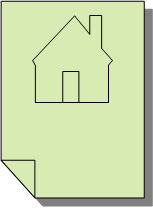
\includegraphics[width=0.25\textwidth]{images/Homepage-icon.png}
  \end{center}
  \caption{Homepage icon}
  \label{fig:homepageicon}
\end{figure}

\begin{table}[!ht]
  \begin{center}
    \caption{Configurations tested}
    \label{tab:configstested}
    \begin{tabular}{l|c} % <-- Alignments: 1st column left, 2nd middle and 3rd right, with vertical lines in between
      \textbf{Configuration} & \textbf{Description} \\
      \hline
      1 & Simple test with one server\\
      2 & Simple test with one server\\
    \end{tabular}
  \end{center}
\end{table}
\todo[inline, backgroundcolor=aqua]{Konfigurationer testade}

\section{Implementation …/Modeling/Simulation/…}
\todo[inline, backgroundcolor=aqua]{Implementering … / modellering / simulering / …}
\label{sec:implementationDetails}

\subsection{Some examples of coding}

Listing~\ref{lst:helloWorldInC} shows an example of a simple program written
in C code.

\begin{lstlisting}[language={C}, caption={Hello world in C code}, label=lst:helloWorldInC]
int main() {
printf("hello, world");
return 0;
}
\end{lstlisting}


In contrast, Listing~\ref{lst:programmes} is an example of code in Python to
get a list of all of the programs at KTH.

\lstset{extendedchars=true}
\begin{lstlisting}[language={Python}, caption={Using a python program to
    access the KTH API to get all of the programs at KTH}, label=lst:programmes]
KOPPSbaseUrl = 'https://www.kth.se'

def v1_get_programmes():
    global Verbose_Flag
    #
    # Use the KOPPS API to get the data
    # note that this returns XML
    url = "{0}/api/kopps/v1/programme".format(KOPPSbaseUrl)
    if Verbose_Flag:
        print("url: " + url)
    #
    r = requests.get(url)
    if Verbose_Flag:
        print("result of getting v1 programme: {}".format(r.text))
    #
    if r.status_code == requests.codes.ok:
        return r.text           # simply return the XML
    #
    return None
\end{lstlisting}
\cleardoublepage
\chapter{Results and Analysis}
\todo[inline, backgroundcolor=aqua]{svensk: Resultat och Analys}
\label{ch:resultsAndAnalysis}
\todo[inline]{
Sometimes this is split into two chapters.\\
  
Keep in mind: How you are going to evaluate what you have done? What are your metrics?\\
Analysis of your data and proposed solution\\
Does this meet the goals which you had when you started?
}

In this chapter, we present the results and discuss them.

\begin{swedishnotes}
I detta kapitel presenterar vi resultatet och diskutera dem.
\end{swedishnotes}
\todo[inline, backgroundcolor=aqua]{
Ibland delas detta upp i två kapitel.\\
Hur du ska utvärdera vad du har gjort? Vad är din statistik?\\
Analys av data och föreslagen lösning\\
Innebär detta att uppnå de mål som du hade när du började?
}

\section{Major results}
\todo[inline, backgroundcolor=aqua]{Huvudsakliga resultat}

Some statistics of the delay measurements are shown in Table~\ref{tab:delayMeasurements}.
The delay has been computed from the time the GET request is received until the response is sent.

\begin{swedishnotes}
Lite statistik av mätningarna fördröjnings visas i Tabell~\ref{tab:delayMeasurements}. Förseningen har beräknats från den tidpunkt då begäran GET tas emot fram till svaret skickas.
\end{swedishnotes}

\begin{table}[!ht]
  \begin{center}
    \caption{Delay measurement statistics}
    \label{tab:delayMeasurements}
    \begin{tabular}{l|S[table-format=4.2]|S[table-format=3.2]} % <-- Alignments: 1st column left, 2nd middle and 3rd right, with vertical lines in between
      \textbf{Configuration} & \textbf{Average delay (ns)} & \textbf{Median delay (ns)}\\
      \hline
      1 & 467.35 & 450.10\\
      2 & 1687.5 & 901.23\\
    \end{tabular}
  \end{center}
\end{table}
\todo[inline, backgroundcolor=aqua]{Fördröj mätstatistik}
\todo[inline, backgroundcolor=aqua]{Konfiguration | Genomsnittlig fördröjning (ns) | Median fördröjning (ns)}

Figure \ref{fig:processing_vs_payload_length} shows and example of the
performance as measured in the experiments.

\begin{figure}[!ht]
% GNUPLOT: LaTeX picture
\setlength{\unitlength}{0.240900pt}
\ifx\plotpoint\undefined\newsavebox{\plotpoint}\fi
\begin{picture}(1500,900)(0,0)
\sbox{\plotpoint}{\rule[-0.200pt]{0.400pt}{0.400pt}}%
\put(171.0,131.0){\rule[-0.200pt]{4.818pt}{0.400pt}}
\put(151,131){\makebox(0,0)[r]{ 1.5}}
\put(1419.0,131.0){\rule[-0.200pt]{4.818pt}{0.400pt}}
\put(171.0,212.0){\rule[-0.200pt]{4.818pt}{0.400pt}}
\put(151,212){\makebox(0,0)[r]{ 2}}
\put(1419.0,212.0){\rule[-0.200pt]{4.818pt}{0.400pt}}
\put(171.0,292.0){\rule[-0.200pt]{4.818pt}{0.400pt}}
\put(151,292){\makebox(0,0)[r]{ 2.5}}
\put(1419.0,292.0){\rule[-0.200pt]{4.818pt}{0.400pt}}
\put(171.0,373.0){\rule[-0.200pt]{4.818pt}{0.400pt}}
\put(151,373){\makebox(0,0)[r]{ 3}}
\put(1419.0,373.0){\rule[-0.200pt]{4.818pt}{0.400pt}}
\put(171.0,454.0){\rule[-0.200pt]{4.818pt}{0.400pt}}
\put(151,454){\makebox(0,0)[r]{ 3.5}}
\put(1419.0,454.0){\rule[-0.200pt]{4.818pt}{0.400pt}}
\put(171.0,534.0){\rule[-0.200pt]{4.818pt}{0.400pt}}
\put(151,534){\makebox(0,0)[r]{ 4}}
\put(1419.0,534.0){\rule[-0.200pt]{4.818pt}{0.400pt}}
\put(171.0,615.0){\rule[-0.200pt]{4.818pt}{0.400pt}}
\put(151,615){\makebox(0,0)[r]{ 4.5}}
\put(1419.0,615.0){\rule[-0.200pt]{4.818pt}{0.400pt}}
\put(171.0,695.0){\rule[-0.200pt]{4.818pt}{0.400pt}}
\put(151,695){\makebox(0,0)[r]{ 5}}
\put(1419.0,695.0){\rule[-0.200pt]{4.818pt}{0.400pt}}
\put(171.0,776.0){\rule[-0.200pt]{4.818pt}{0.400pt}}
\put(151,776){\makebox(0,0)[r]{ 5.5}}
\put(1419.0,776.0){\rule[-0.200pt]{4.818pt}{0.400pt}}
\put(171.0,131.0){\rule[-0.200pt]{0.400pt}{4.818pt}}
\put(171,90){\makebox(0,0){ 0}}
\put(171.0,756.0){\rule[-0.200pt]{0.400pt}{4.818pt}}
\put(298.0,131.0){\rule[-0.200pt]{0.400pt}{4.818pt}}
\put(298,90){\makebox(0,0){ 10}}
\put(298.0,756.0){\rule[-0.200pt]{0.400pt}{4.818pt}}
\put(425.0,131.0){\rule[-0.200pt]{0.400pt}{4.818pt}}
\put(425,90){\makebox(0,0){ 20}}
\put(425.0,756.0){\rule[-0.200pt]{0.400pt}{4.818pt}}
\put(551.0,131.0){\rule[-0.200pt]{0.400pt}{4.818pt}}
\put(551,90){\makebox(0,0){ 30}}
\put(551.0,756.0){\rule[-0.200pt]{0.400pt}{4.818pt}}
\put(678.0,131.0){\rule[-0.200pt]{0.400pt}{4.818pt}}
\put(678,90){\makebox(0,0){ 40}}
\put(678.0,756.0){\rule[-0.200pt]{0.400pt}{4.818pt}}
\put(805.0,131.0){\rule[-0.200pt]{0.400pt}{4.818pt}}
\put(805,90){\makebox(0,0){ 50}}
\put(805.0,756.0){\rule[-0.200pt]{0.400pt}{4.818pt}}
\put(932.0,131.0){\rule[-0.200pt]{0.400pt}{4.818pt}}
\put(932,90){\makebox(0,0){ 60}}
\put(932.0,756.0){\rule[-0.200pt]{0.400pt}{4.818pt}}
\put(1059.0,131.0){\rule[-0.200pt]{0.400pt}{4.818pt}}
\put(1059,90){\makebox(0,0){ 70}}
\put(1059.0,756.0){\rule[-0.200pt]{0.400pt}{4.818pt}}
\put(1185.0,131.0){\rule[-0.200pt]{0.400pt}{4.818pt}}
\put(1185,90){\makebox(0,0){ 80}}
\put(1185.0,756.0){\rule[-0.200pt]{0.400pt}{4.818pt}}
\put(1312.0,131.0){\rule[-0.200pt]{0.400pt}{4.818pt}}
\put(1312,90){\makebox(0,0){ 90}}
\put(1312.0,756.0){\rule[-0.200pt]{0.400pt}{4.818pt}}
\put(1439.0,131.0){\rule[-0.200pt]{0.400pt}{4.818pt}}
\put(1439,90){\makebox(0,0){ 100}}
\put(1439.0,756.0){\rule[-0.200pt]{0.400pt}{4.818pt}}
\put(171.0,131.0){\rule[-0.200pt]{0.400pt}{155.380pt}}
\put(171.0,131.0){\rule[-0.200pt]{305.461pt}{0.400pt}}
\put(1439.0,131.0){\rule[-0.200pt]{0.400pt}{155.380pt}}
\put(171.0,776.0){\rule[-0.200pt]{305.461pt}{0.400pt}}
\put(30,453){\rotatebox{-270}{\makebox(0,0){Processing time (ms)}}}
\put(805,29){\makebox(0,0){Payload size (bytes)}}
\put(868.0,131.0){\rule[-0.200pt]{0.400pt}{84.074pt}}
\put(995.0,131.0){\rule[-0.200pt]{0.400pt}{98.287pt}}
\put(1173.0,131.0){\rule[-0.200pt]{0.400pt}{118.041pt}}
\put(1325.0,131.0){\rule[-0.200pt]{0.400pt}{134.904pt}}
\put(1350.0,131.0){\rule[-0.200pt]{0.400pt}{137.795pt}}
\put(1439.0,131.0){\rule[-0.200pt]{0.400pt}{155.380pt}}
\end{picture}
\caption[A GNUplot figure]{Processing time vs. payload length}\vspace{0.5cm}
\label{fig:processing_vs_payload_length}
\end{figure}
		

Given these measurements, we can calculate our processing bit rate as the inverse of the time it takes to process an additional byte divided by 8 bits per byte:

\[
	bitrate = \frac{1}{\frac{time_{byte}}{8}} = 20.03 \quad kb/s
\] 

\section{Reliability Analysis}
\todo[inline, backgroundcolor=aqua]{Analys av reabilitet}
\begin{swedishnotes}
Reabilitet i metod och data 
\end{swedishnotes}

\section{Validity Analysis}
\todo[inline, backgroundcolor=aqua]{Analys av validitet}
\begin{swedishnotes}
Validitet i metod och data 
\end{swedishnotes}\cleardoublepage
\chapter{Discussion}\todo[inline]{This can be a separate chapter or a section
  in the previous chapter.}
\todo[inline, backgroundcolor=aqua]{Diskussion}
\label{ch:discussion}
\begin{swedishnotes}
Förbättringsförslag?
\end{swedishnotes}

\cleardoublepage
\chapter{Conclusions and Future work}
\todo[inline, backgroundcolor=aqua]{Slutsats och framtida arbete}
\label{ch:conclusionsAndFutureWork}
Add text to introduce the subsections of this chapter.

\section{Conclusions}
\todo[inline]{Describe the conclusions (reflect on the whole introduction given in Chapter 1).}
\todo[inline, backgroundcolor=aqua]{Slutsatser}
\label{sec:conclusions}
  
Discuss the positive effects and the drawbacks.\\
Describe the evaluation of the results of the degree project.\\
Did you meet your goals?\\
What insights have you gained?\\
What suggestions can you give to others working in this area?\\
If you had it to do again, what would you have done differently?\\

\begin{swedishnotes}
Träffade du dina mål?
Vilka insikter har du fått?
Vilka förslag kan du ge till andra som arbetar inom detta område?
Om du hade att göra igen, vad skulle du ha gjort annorlunda?
\end{swedishnotes}

\section{Limitations}
\todo[inline]{What did you find that limited your
  efforts? What are the limitations of your results?}
\todo[inline, backgroundcolor=aqua]{Begränsande faktorer}
\label{sec:limitations}
\begin{swedishnotes}
Vad gjorde du som begränsade dina ansträngningar? Vilka är begränsningarna i dina resultat?
\end{swedishnotes}

\section{Future work}
\todo[inline]{Describe valid future work that you or someone else could or should do.\\
Consider: What you have left undone? What are the next obvious things to be done? What hints can you give to the next person who is going to follow up on your work?
}
\todo[inline, backgroundcolor=aqua]{Vad du har kvar ogjort?\\
Vad är nästa självklara saker som ska göras?\\
Vad tips kan du ge till nästa person som kommer att följa upp på ditt arbete?
}
\label{sec:futureWork}

Due to the breadth of the problem, only some of the initial goals have been
met. In these section we will focus on some of the remaining issues that
should be addressed in future work. ...

\subsection{What has been left undone?}
\label{what-has-been-left-undone}

The prototype does not address the third requirment, i.e., a yearly
unavailability of less than 3 minutes, this remains an open problem. ...

\subsubsection{Cost analysis}

The current prototype works, but the performance from a cost perspective makes
this an impractical solution. Future work must reduce the cost of this
solution, to do so a cost analysis needs to first be done. ...

\subsubsection{Security}

A future research effort is needed to address the security holes that results
from using a self-signed certificate. Page filling text mass. Page filling
text mass. ...


\subsection{Next obvious things to be done}

In particular, the author of this thesis wishes to point out xxxxxx remains as
a problem to be solved. Solving this problem is the next thing that should be
done. ...

\section{Reflections}
\todo[inline]{What are the relevant economic, social,
  environmental, and ethical aspects of your work?
}
\todo[inline, backgroundcolor=aqua]{Reflektioner}
\todo[inline, backgroundcolor=aqua]{Vilka är de relevanta ekonomiska, sociala, miljömässiga och etiska aspekter av ditt arbete?}
\label{sec:reflections}

One of the most important results is the reduction in the amount of
energy required to process each packet while at the same time reducing the
time required to process each packet.

The thesis contributes to the \gls{UN}\enspace\glspl{SDG} numbers 1 and 9 by
xxxx. 

\noindent\rule{\textwidth}{0.4mm}\cleardoublepage

\bibliographystyle{myIEEEtran}
\renewcommand{\bibname}{References}
\addcontentsline{toc}{chapter}{References}
\bibliography{references}

\cleardoublepage
\appendix
\renewcommand{\chaptermark}[1]{\markboth{Appendix \thechapter\relax:\thinspace\relax#1}{}}
\chapter{Something Extra}

\label{pg:lastPageofMainmatter}

\clearpage
\section*{For DIVA}
\divainfo{pg:lastPageofPreface}{pg:lastPageofMainmatter}

\end{document}
